%форматирование размера документа
\documentclass[11pt, a4paper]{article}

\usepackage{geometry}
% total - determines printable width, height
\geometry{ 
	a4paper, total={180mm,267mm}
}

%----text,fonts------------------------------------------------------------------------------------
\usepackage{mmap}
\usepackage[T2A]{fontenc}
\usepackage[utf8]{inputenc}
\usepackage[english, russian]{babel}
\usepackage{setspace}
\setstretch{0,9}
\usepackage{fancyvrb}

%----math,graphics---------------------------------------------------------------------------------
\usepackage{amsmath,amsfonts,amssymb}
\usepackage{amsthm}
\usepackage{listings}
\usepackage{xcolor}
\usepackage{filecontents}
\usepackage{fancyvrb}
\usepackage{fvextra}
\usepackage{hyperref}
\hypersetup{
    colorlinks=true,
    linkcolor=blue,
    filecolor=magenta,      
    urlcolor=blue,
    pdftitle={Overleaf Example},
    pdfpagemode=FullScreen,
}

\usepackage{tikz}
\usetikzlibrary{calc}
\usepackage{pgfplots}
\pgfplotsset{
	compat=1.17
}

\usepackage{graphicx}
\graphicspath{{images/}}
  
\usepackage{wrapfig}
\usepackage{tabularx}

% relative importing
\usepackage{import}

% % --- ugly internals for language definition ---
%
\makeatletter

% initialisation of user macros
\newcommand\PrologPredicateStyle{}
\newcommand\PrologVarStyle{}
\newcommand\PrologAnonymVarStyle{}
\newcommand\PrologAtomStyle{}
\newcommand\PrologOtherStyle{}
\newcommand\PrologCommentStyle{}

% useful switches (to keep track of context)
\newif\ifpredicate@prolog@
\newif\ifwithinparens@prolog@

% save definition of underscore for test
\lst@SaveOutputDef{`_}\underscore@prolog

% local variables
\newcount\currentchar@prolog

\newcommand\@testChar@prolog%
{%
  % if we're in processing mode...
  \ifnum\lst@mode=\lst@Pmode%
    \detectTypeAndHighlight@prolog%
  \else
    % ... or within parentheses
    \ifwithinparens@prolog@%
      \detectTypeAndHighlight@prolog%
    \fi
  \fi
  % Some housekeeping...
  \global\predicate@prolog@false%
}

% helper macros
\newcommand\detectTypeAndHighlight@prolog
{%
  % First, assume that we have an atom.
  \def\lst@thestyle{\PrologAtomStyle}%
  % Test whether we have a predicate and modify the style accordingly.
  \ifpredicate@prolog@%
    \def\lst@thestyle{\PrologPredicateStyle}%
  \else
    % Test whether we have a predicate and modify the style accordingly.
    \expandafter\splitfirstchar@prolog\expandafter{\the\lst@token}%
    % Check whether the identifier starts by an underscore.
    \expandafter\ifx\@testChar@prolog\underscore@prolog%
      % Check whether the identifier is '_' (anonymous variable)
      \ifnum\lst@length=1%
        \let\lst@thestyle\PrologAnonymVarStyle%
      \else
        \let\lst@thestyle\PrologVarStyle%
      \fi
    \else
      % Check whether the identifier starts by a capital letter.
      \currentchar@prolog=65
      \loop
        \expandafter\ifnum\expandafter`\@testChar@prolog=\currentchar@prolog%
          \let\lst@thestyle\PrologVarStyle%
          \let\iterate\relax
        \fi
        \advance \currentchar@prolog by 1
        \unless\ifnum\currentchar@prolog>90
      \repeat
    \fi
  \fi
}
\newcommand\splitfirstchar@prolog{}
\def\splitfirstchar@prolog#1{\@splitfirstchar@prolog#1\relax}
\newcommand\@splitfirstchar@prolog{}
\def\@splitfirstchar@prolog#1#2\relax{\def\@testChar@prolog{#1}}

% helper macro for () delimiters
\def\beginlstdelim#1#2%
{%
  \def\endlstdelim{\PrologOtherStyle #2\egroup}%
  {\PrologOtherStyle #1}%
  \global\predicate@prolog@false%
  \withinparens@prolog@true%
  \bgroup\aftergroup\endlstdelim%
}

% language name
\newcommand\lang@prolog{Prolog-pretty}
% ``normalised'' language name
\expandafter\lst@NormedDef\expandafter\normlang@prolog%
  \expandafter{\lang@prolog}

% language definition
\expandafter\expandafter\expandafter\lstdefinelanguage\expandafter%
{\lang@prolog}
{%
  language            = Prolog,
  keywords            = {},      % reset all preset keywords
  showstringspaces    = false,
  alsoletter          = (,
  alsoother           = @$,
  moredelim           = **[is][\beginlstdelim{(}{)}]{(}{)},
  MoreSelectCharTable =
    \lst@DefSaveDef{`(}\opparen@prolog{\global\predicate@prolog@true\opparen@prolog},
}

% Hooking into listings to test each ``identifier''
\newcommand\@ddedToOutput@prolog\relax
\lst@AddToHook{Output}{\@ddedToOutput@prolog}

\lst@AddToHook{PreInit}
{%
  \ifx\lst@language\normlang@prolog%
    \let\@ddedToOutput@prolog\@testChar@prolog%
  \fi
}

\lst@AddToHook{DeInit}{\renewcommand\@ddedToOutput@prolog{}}

\makeatother
%
% --- end of ugly internals ---


% --- definition of a custom style similar to that of Pygments ---
% custom colors
\definecolor{PrologPredicate}{RGB}{000,031,255}
\definecolor{PrologVar}      {RGB}{024,021,125}
\definecolor{PrologAnonymVar}{RGB}{000,127,000}
\definecolor{PrologAtom}     {RGB}{186,032,032}
\definecolor{PrologComment}  {RGB}{063,128,127}
\definecolor{PrologOther}    {RGB}{000,000,000}

% redefinition of user macros for Prolog style
\renewcommand\PrologPredicateStyle{\color{PrologPredicate}}
\renewcommand\PrologVarStyle{\color{PrologVar}}
\renewcommand\PrologAnonymVarStyle{\color{PrologAnonymVar}}
\renewcommand\PrologAtomStyle{\color{PrologAtom}}
\renewcommand\PrologCommentStyle{\itshape\color{PrologComment}}
\renewcommand\PrologOtherStyle{\color{PrologOther}}

% custom style definition 
\lstdefinestyle{Prolog-pygsty}
{
  language     = Prolog-pretty,
  upquote      = true,
  stringstyle  = \PrologAtomStyle,
  commentstyle = \PrologCommentStyle,
  literate     =
    {:-}{{\PrologOtherStyle :-}}2
    {,}{{\PrologOtherStyle ,}}1
    {.}{{\PrologOtherStyle .}}1
}

% global settings
\lstset
{
  captionpos = below,
  frame      = single,
  columns    = fullflexible,
  basicstyle = \ttfamily,
}


\begin{document}

\import{.}{titular.tex}

\newpage

\section{Текст задания}
\noindentОсновная цель лабораторной работы - знакомство с системными инструментами анализа производительности и поведения программ. Для этого предлагается для выданной по варианту программы выяснить следующую информацию:

\begin{enumerate}
  \item Количество потоков создаваемое программой;
  \item Список файлов и сетевых соединений с которыми работает программа
  \item Карту памяти процесса;
  \item Содержимое передаваемых по сети данных;
  \item Построить графики:
  \begin{itemize}
    \item Потребления программой cpu;
    \item Нагрузки генерируемой программой на подсистему ввода-вывода;
    \item Нагрузки генерируемой программой на сетевую подсистему.
    \item Смены состояния исполнения потоков;
  \end{itemize}
\end{enumerate}

\smallskip

\noindentСодержание отчета:
\begin{enumerate}
  \item Описание шагов выполненных для сбора информации (включая исходные тексты всех использованных скриптов и вспомогательных программ);
  \item  Полученные графики;
  \item  Выводы по работе.
\end{enumerate}

\noindentТемы для подготовки к защите лабораторной работы:
\begin{enumerate}
  \item Структура процесса;
  \item Виртуальная память;
  \item Системные утилиты сбора статистики ядра;
  \item Основы ввода-вывода (блочный и последовательный ввод-вывод);
  \item Файловая система procfs;
  \item Использование утилиты strace, ltrace, bpftrace;
  \item Профилирование и построение flamegraph'а и stap;
\end{enumerate}

\section{Выполнение}

% \begin{Verbatim}[fontsize=\small]
% Список утилит:

% Процессор: ps, top, tiptop, turbostat, rdmsr, numastat, uptime, mpstat,

% Виртуальная память: vmstat, slabtop, pidstat, free, pcstat, lsof

% Дисковая подсистема: iostat, iotop, blktrace, swapon

% Сеть: netstat, tcpdump, iptraf, ethtool, nicstat, ip, lldptool, snmpget, ss

% System calls: sysdig, strace

% Library calls: ltrace

% Другое: sar, perf, dstat, dmesg, bcc, lttng, stap, ftrace

% \end{Verbatim}

\subsection{Количество потоков создаваемое программой}
Посчитаем уникальных \$SPID (идентификатор потока) у запущенного процесса:
\begin{Verbatim}[fontsize=\small]
nikit@vm:~$ ps -T -p 4098
    PID    SPID TTY          TIME CMD
   4098    4098 pts/0    00:00:00 256771
   4098    4099 pts/0    00:00:05 256771
   4098    4100 pts/0    00:00:03 256771
   4098    4101 pts/0    00:00:05 256771
   4098    4102 pts/0    00:00:03 256771
   4098    4103 pts/0    00:00:05 256771
   4098    4104 pts/0    00:00:03 256771
   4098    4105 pts/0    00:00:05 256771
   4098    4106 pts/0    00:00:03 256771
   4098    4107 pts/0    00:00:00 256771
   4098    4108 pts/0    00:00:00 256771
   4098    4109 pts/0    00:00:00 256771
   4098    4110 pts/0    00:00:00 256771
   4098    4111 pts/0    00:00:00 256771
   4098    4112 pts/0    00:00:00 256771
   4098    4113 pts/0    00:00:00 256771
   4098    4114 pts/0    00:00:00 256771
   4098    4115 pts/0    00:00:00 256771
   4098    4116 pts/0    00:00:00 256771
   4098    4117 pts/0    00:00:00 256771
   4098    4118 pts/0    00:00:00 256771
   4098    4119 pts/0    00:00:11 256771
   4098    4120 pts/0    00:00:39 256771
   4098    4121 pts/0    00:00:39 256771

nikit@vm:~$ echo "$(($(ps -T -p 4098 | wc -l) - 1))"
24

nikit@vm:~$ top -H -p 4098
top - 11:25:38 up 50 min,  2 users,  load average: 1.16, 1.09, 0.73
Threads:  24 total,   1 running,  23 sleeping,   0 stopped,   0 zombie
%Cpu(s):  6.9 us, 19.2 sy,  0.0 ni, 72.0 id,  1.5 wa,  0.0 hi,  0.3 si,  0.0 st
MiB Mem :   3931.1 total,   1717.5 free,    855.1 used,   1358.5 buff/cache
MiB Swap:    975.0 total,    975.0 free,      0.0 used.   2799.7 avail Mem

    PID USER      PR  NI    VIRT    RES    SHR S  %CPU  %MEM     TIME+ COMMAND
   4099 nikit     20   0 1652680 772196   3092 S  30.9  19.2   0:13.28 256771
   4105 nikit     20   0 1652680 772196   3092 R  29.6  19.2   0:13.54 256771
   4120 nikit     20   0 1652680 774244   3092 S  13.0  19.2   1:56.40 256771
   4121 nikit     20   0 1652680 774244   3092 S  13.0  19.2   1:56.51 256771
   4100 nikit     20   0 1652680 772196   3092 S  10.3  19.2   0:10.21 256771
   4104 nikit     20   0 1652680 772196   3092 S   3.7  19.2   0:10.39 256771
   4106 nikit     20   0 1652680 772196   3092 S   3.0  19.2   0:10.28 256771
   4102 nikit     20   0 1652680 772196   3092 S   2.7  19.2   0:10.20 256771
   4098 nikit     20   0 1652680 772196   3092 S   0.0  19.2   0:00.00 256771
   4101 nikit     20   0 1652680 772196   3092 S   0.0  19.2   0:13.96 256771
   4103 nikit     20   0 1652680 772196   3092 S   0.0  19.2   0:14.17 256771
   4107 nikit     20   0 1652680 772196   3092 S   0.0  19.2   0:00.00 256771
   4108 nikit     20   0 1652680 774244   3092 S   0.0  19.2   0:00.01 256771
   4109 nikit     20   0 1652680 774244   3092 S   0.0  19.2   0:00.00 256771
   4110 nikit     20   0 1652680 774244   3092 S   0.0  19.2   0:00.02 256771
   4111 nikit     20   0 1652680 774244   3092 S   0.0  19.2   0:00.00 256771
   4112 nikit     20   0 1652680 774244   3092 S   0.0  19.2   0:00.02 256771
   4113 nikit     20   0 1652680 774244   3092 S   0.0  19.2   0:00.00 256771
   4114 nikit     20   0 1652680 774244   3092 S   0.0  19.2   0:00.01 256771
   4115 nikit     20   0 1652680 774244   3092 S   0.0  19.2   0:00.00 256771
   4116 nikit     20   0 1652680 774244   3092 S   0.0  19.2   0:00.02 256771
   4117 nikit     20   0 1652680 774244   3092 S   0.0  19.2   0:00.00 256771
   4118 nikit     20   0 1652680 774244   3092 S   0.0  19.2   0:00.02 256771
   4119 nikit     20   0 1652680 774244   3092 S   0.0  19.2   0:31.66 256771
\end{Verbatim}

\newpage
С помощью htop:

\begin{figure}[h]
  \centering
  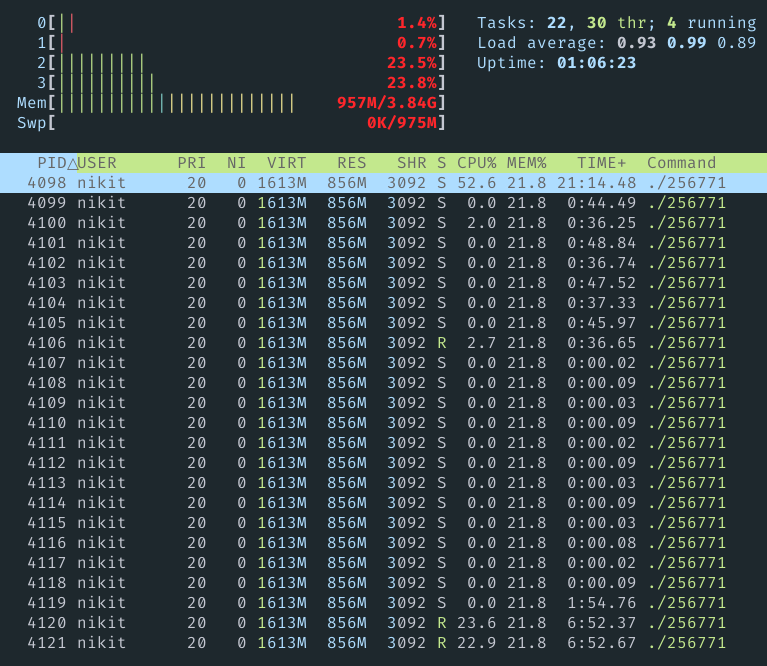
\includegraphics[width=0.7\textwidth]{htop-1.png}
  % \label{fig:result-png}
\end{figure}


\subsection{Список файлов и сетевых соединений с которыми работает программа}
\begin{Verbatim}[fontsize=\small,breaklines=true]
nikit@vm:~$ ls -la /proc/4098/fd/
total 0
dr-x------ 2 nikit nikit  0 Sep 25 11:19 .
dr-xr-xr-x 9 nikit nikit  0 Sep 25 11:19 ..
lrwx------ 1 nikit nikit 64 Sep 25 11:19 0 -> /dev/pts/0
lrwx------ 1 nikit nikit 64 Sep 25 11:19 1 -> /dev/pts/0
lrwx------ 1 nikit nikit 64 Sep 25 11:19 2 -> /dev/pts/0
lrwx------ 1 nikit nikit 64 Sep 25 11:19 3 -> 'socket:[34028]'
lrwx------ 1 nikit nikit 64 Sep 25 11:19 6 -> 'socket:[34913]'
lrwx------ 1 nikit nikit 64 Sep 25 11:19 8 -> 'socket:[34029]'


nikit@vm:~$ lsof -p 4098
COMMAND  PID  USER   FD   TYPE DEVICE SIZE/OFF   NODE NAME
256771  4098 nikit  cwd    DIR    8,1     4096 397903 /home/nikit/labs/os-1
256771  4098 nikit  rtd    DIR    8,1     4096      2 /
256771  4098 nikit  txt    REG    8,1   224160 397902 /home/nikit/labs/os-1/256771
256771  4098 nikit  mem    REG    8,1  1905632 783386 /usr/lib/x86_64-linux-gnu/libc-2.31.so
256771  4098 nikit  mem    REG    8,1   149520 784083 /usr/lib/x86_64-linux-gnu/libpthread-2.31.so
256771  4098 nikit  mem    REG    8,1   100736 783371 /usr/lib/x86_64-linux-gnu/libgcc_s.so.1
256771  4098 nikit  mem    REG    8,1  1321344 784071 /usr/lib/x86_64-linux-gnu/libm-2.31.so
256771  4098 nikit  mem    REG    8,1  1870824 786723 /usr/lib/x86_64-linux-gnu/libstdc++.so.6.0.28
256771  4098 nikit  mem    REG    8,1   177928 783381 /usr/lib/x86_64-linux-gnu/ld-2.31.so
256771  4098 nikit    0u   CHR  136,0      0t0      3 /dev/pts/0
256771  4098 nikit    1u   CHR  136,0      0t0      3 /dev/pts/0
256771  4098 nikit    2u   CHR  136,0      0t0      3 /dev/pts/0
256771  4098 nikit    4u  sock    0,8      0t0  35032 protocol: TCP
256771  4098 nikit    5u  sock    0,8      0t0  32426 protocol: TCP


# Через strace (основные данные):
nikit@vm:~/labs/os-1/task$ strace -f -e open,openat,creat -o strace-1.log ./256771
# Вывод (* - все внутри директории)

# Загружаем библиотеки
1953  openat(AT_FDCWD, "/etc/ld.so.cache", O_RDONLY|O_CLOEXEC) = 3
1953  openat(AT_FDCWD, "/lib/x86_64-linux-gnu/libstdc++.so.6", O_RDONLY|O_CLOEXEC) = 3
1953  openat(AT_FDCWD, "/lib/x86_64-linux-gnu/libm.so.6", O_RDONLY|O_CLOEXEC) = 3
1953  openat(AT_FDCWD, "/lib/x86_64-linux-gnu/libgcc_s.so.1", O_RDONLY|O_CLOEXEC) = 3
1953  openat(AT_FDCWD, "/lib/x86_64-linux-gnu/libpthread.so.0", O_RDONLY|O_CLOEXEC) = 3
1953  openat(AT_FDCWD, "/lib/x86_64-linux-gnu/libc.so.6", O_RDONLY|O_CLOEXEC) = 3
1954  openat(AT_FDCWD, "/dev/urandom", O_RDONLY) = 3

# Далее рекурсивный обход proc (все файлы, название которых не pid; self/task/$PID для каждого процесса и треда):
1974  openat(AT_FDCWD, "/proc", O_RDONLY|O_NONBLOCK|O_CLOEXEC|O_DIRECTORY) = 13
1974  openat(AT_FDCWD, "/proc/fs", O_RDONLY|O_NONBLOCK|O_CLOEXEC|O_DIRECTORY) = 18
1974  openat(AT_FDCWD, "/proc/fs/ext4", O_RDONLY|O_NONBLOCK|O_CLOEXEC|O_DIRECTORY) = 18
1974  openat(AT_FDCWD, "/proc/fs/ext4/sda1", O_RDONLY|O_NONBLOCK|O_CLOEXEC|O_DIRECTORY) = 18
1974  openat(AT_FDCWD, "/proc/fs/jbd2", O_RDONLY|O_NONBLOCK|O_CLOEXEC|O_DIRECTORY) = 18
1974  openat(AT_FDCWD, "/proc/fs/jbd2/sda1-8", O_RDONLY|O_NONBLOCK|O_CLOEXEC|O_DIRECTORY) = 18
1974  openat(AT_FDCWD, "/proc/fs/nfsd", O_RDONLY|O_NONBLOCK|O_CLOEXEC|O_DIRECTORY) = 18
1974  openat(AT_FDCWD, "/proc/bus", O_RDONLY|O_NONBLOCK|O_CLOEXEC|O_DIRECTORY) = 18
1974  openat(AT_FDCWD, "/proc/bus/pci", O_RDONLY|O_NONBLOCK|O_CLOEXEC|O_DIRECTORY) = 18
1974  openat(AT_FDCWD, "/proc/bus/pci/00", O_RDONLY|O_NONBLOCK|O_CLOEXEC|O_DIRECTORY) = 18
1974  openat(AT_FDCWD, "/proc/bus/input", O_RDONLY|O_NONBLOCK|O_CLOEXEC|O_DIRECTORY) = 18
1974  openat(AT_FDCWD, "/proc/irq", O_RDONLY|O_NONBLOCK|O_CLOEXEC|O_DIRECTORY) = 18
1974  openat(AT_FDCWD, "/proc/irq/0", O_RDONLY|O_NONBLOCK|O_CLOEXEC|O_DIRECTORY) = 18
...
1974  openat(AT_FDCWD, "/proc/self/task/1953/root/lib/modules/5.10.0-18-amd64/kernel/drivers/net/ethernet/mellanox/mlxfw", O_RDONLY|O_NONBLOCK|O_CLOEXEC|O_DIRECTORY) = 3
1974  openat(AT_FDCWD, "/proc/self/task/1954", O_RDONLY|O_NONBLOCK|O_CLOEXEC|O_DIRECTORY) = 4
1974  openat(AT_FDCWD, "/proc/self/task/1954/fd", O_RDONLY|O_NONBLOCK|O_CLOEXEC|O_DIRECTORY) = 4
1974  openat(AT_FDCWD, "/proc/self/task/1954/fdinfo", O_RDONLY|O_NONBLOCK|O_CLOEXEC|O_DIRECTORY) = 4
1974  openat(AT_FDCWD, "/proc/self/task/1954/ns", O_RDONLY|O_NONBLOCK|O_CLOEXEC|O_DIRECTORY) = 4
1974  openat(AT_FDCWD, "/proc/self/task/1954/net", O_RDONLY|O_NONBLOCK|O_CLOEXEC|O_DIRECTORY) = 4
1974  openat(AT_FDCWD, "/proc/self/task/1954/attr", O_RDONLY|O_NONBLOCK|O_CLOEXEC|O_DIRECTORY) = 4
1974  openat(AT_FDCWD, "/proc/self/task/1954/attr/apparmor", O_RDONLY|O_NONBLOCK|O_CLOEXEC|O_DIRECTORY) = 4
1974  openat(AT_FDCWD, "/proc/self/task/1955", O_RDONLY|O_NONBLOCK|O_CLOEXEC|O_DIRECTORY) = 4
1974  openat(AT_FDCWD, "/proc/self/task/1955/fd", O_RDONLY|O_NONBLOCK|O_CLOEXEC|O_DIRECTORY) = 4
1974  openat(AT_FDCWD, "/proc/self/task/1955/fdinfo", O_RDONLY|O_NONBLOCK|O_CLOEXEC|O_DIRECTORY) = 4
...
# Далее открываем файлики с цифрами в директории исполняемого бинарника:
1956  openat(AT_FDCWD, "8166219804254678425", O_WRONLY|O_CREAT|O_TRUNC, 0666) = 3
1956  openat(AT_FDCWD, "8166219804254678425", O_RDONLY) = 3
1956  openat(AT_FDCWD, "8166219804254678425", O_RDONLY) = 3
1957  openat(AT_FDCWD, "12064446664900734791", O_WRONLY|O_CREAT|O_TRUNC, 0666) = 4
1960  openat(AT_FDCWD, "/dev/urandom", O_RDONLY) = 3
1954  openat(AT_FDCWD, "/dev/urandom", O_RDONLY) = 4
1958  openat(AT_FDCWD, "/dev/urandom", O_RDONLY) = 5
1954  openat(AT_FDCWD, "13817306382609589397", O_WRONLY|O_CREAT|O_TRUNC, 0666 <unfinished ...>
1960  openat(AT_FDCWD, "16618435859175486135", O_WRONLY|O_CREAT|O_TRUNC, 0666) = 3
1954  <... openat resumed>)             = 4
1958  openat(AT_FDCWD, "15233208405822243171", O_WRONLY|O_CREAT|O_TRUNC, 0666) = 5
1960  openat(AT_FDCWD, "16618435859175486135", O_RDONLY) = 3
1960  openat(AT_FDCWD, "16618435859175486135", O_RDONLY) = 3
1961  openat(AT_FDCWD, "9709491411073380223", O_WRONLY|O_CREAT|O_TRUNC, 0666) = 4
1954  openat(AT_FDCWD, "13817306382609589397", O_RDONLY) = 3
1954  openat(AT_FDCWD, "13817306382609589397", O_RDONLY) = 3
1955  openat(AT_FDCWD, "14069912073054239648", O_WRONLY|O_CREAT|O_TRUNC, 0666) = 9
1958  openat(AT_FDCWD, "15233208405822243171", O_RDONLY) = 3
1958  openat(AT_FDCWD, "15233208405822243171", O_RDONLY) = 3
1959  openat(AT_FDCWD, "2858444524433567647", O_WRONLY|O_CREAT|O_TRUNC, 0666) = 3

# Цикл начинается с начала по кругу 
\end{Verbatim}

% \begin{Verbatim}
% FD         is the File Descriptor number of the file or:
%      cwd  current working directory;
%      Lnn  library references (AIX);
%      err  FD information error (see NAME column);
%      jld  jail directory (FreeBSD);
%      ltx  shared library text (code and data);
%      Mxx  hex memory-mapped type number xx.
%      m86  DOS Merge mapped file;
%      mem  memory-mapped file;
%      mmap memory-mapped device;
%      pd   parent directory;
%      rtd  root directory;
%      tr   kernel trace file (OpenBSD);
%      txt  program text (code and data);
%      v86  VP/ix mapped file;

% FD is followed by one of these characters, describing the mode under  which
% the file is open:
%      r for read access;
%      w for write access;
%      u for read and write access;
%      space if mode unknown and no lock
%           character follows;
%      `-' if mode unknown and lock
%           character follows.
% \end{Verbatim}

\subsection{Карта памяти процесса}
Можно использовать ключик -X или -XX для большего кол-ва информации (там флаги страничек).

% \begin{itemize}
%   \item Resident set size (RSS) — размер страниц памяти, выделенных процессу операционной системой и в настоящее время находящихся в ОЗУ (RAM).
%   \item Pages in the page cache modified after being brought in are called dirty pages. Когда программа делает вызов write(), данные просто копируются в соответствующую страницу в страничном кэше, и она помечается флагом «dirty».
%   \item The pages are private, not shared, so they wouldn't be saved back into the original file. It would be impossible to have a dirty page backed by a read-only file. If the page needs to be removed from RAM, it will be saved in swap.
% \end{itemize}
\begin{Verbatim}[fontsize=\small]
nikit@vm:~$ pmap -x 4098
4098:   ./256771
Address           Kbytes     RSS   Dirty Mode  Mapping
0000000000400000     216     188       0 r-x-- 256771
0000000000635000       4       4       4 r---- 256771
0000000000636000       4       4       4 rw--- 256771
0000000000777000     132      32      32 rw---   [ anon ]
00007fca51600000  108544  108544  108544 rw---   [ anon ]
00007fca58000000     132       8       8 rw---   [ anon ]
00007fca58021000   65404       0       0 -----   [ anon ]
00007fca60000000     132       8       8 rw---   [ anon ]
00007fca60021000   65404       0       0 -----   [ anon ]
00007fca65600000  108544  108544  108544 rw---   [ anon ]
00007fca6c000000     132       8       8 rw---   [ anon ]
00007fca6c021000   65404       0       0 -----   [ anon ]
00007fca70200000  108544  108544  108544 rw---   [ anon ]
00007fca7d600000  108544  108544  108544 rw---   [ anon ]
00007fca84000000    1876     928     928 rw---   [ anon ]
00007fca841d5000   63660       0       0 -----   [ anon ]
00007fca88000000     132       8       8 rw---   [ anon ]
00007fca88021000   65404       0       0 -----   [ anon ]
00007fca8c000000     132       8       8 rw---   [ anon ]
00007fca8c021000   65404       0       0 -----   [ anon ]
00007fca90000000     132       8       8 rw---   [ anon ]
00007fca90021000   65404       0       0 -----   [ anon ]
00007fca94ffa000       4       0       0 -----   [ anon ]
00007fca94ffb000    8192       8       8 rw---   [ anon ]
00007fca957fb000       4       0       0 -----   [ anon ]
00007fca957fc000    8192       8       8 rw---   [ anon ]
00007fca95ffc000       4       0       0 -----   [ anon ]
00007fca95ffd000    8192      28      28 rw---   [ anon ]
00007fca967fd000       4       0       0 -----   [ anon ]
00007fca967fe000    8192       8       8 rw---   [ anon ]
00007fca96ffe000       4       0       0 -----   [ anon ]
00007fca96fff000    8192       8       8 rw---   [ anon ]
00007fca977ff000       4       0       0 -----   [ anon ]
00007fca97800000    8192    2048    2048 rw---   [ anon ]
00007fca98000000     132       8       8 rw---   [ anon ]
00007fca98021000   65404       0       0 -----   [ anon ]
00007fca9c7f9000       4       0       0 -----   [ anon ]
00007fca9c7fa000    8192       8       8 rw---   [ anon ]
00007fca9cffa000       4       0       0 -----   [ anon ]
00007fca9cffb000    8192       8       8 rw---   [ anon ]
00007fca9d7fb000       4       0       0 -----   [ anon ]
00007fca9d7fc000    8192       8       8 rw---   [ anon ]
00007fca9dffc000       4       0       0 -----   [ anon ]
00007fca9dffd000    8192       8       8 rw---   [ anon ]
00007fca9e7fd000       4       0       0 -----   [ anon ]
00007fca9e7fe000    8192       8       8 rw---   [ anon ]
00007fca9effe000       4       0       0 -----   [ anon ]
00007fca9efff000    8192       8       8 rw---   [ anon ]
00007fca9f7ff000       4       0       0 -----   [ anon ]
00007fca9f800000    8192    2048    2048 rw---   [ anon ]
00007fcaa0000000     132       8       8 rw---   [ anon ]
00007fcaa0021000   65404       0       0 -----   [ anon ]
00007fcaa421d000       4       0       0 -----   [ anon ]
00007fcaa421e000    8192       8       8 rw---   [ anon ]
00007fcaa4a1e000       4       0       0 -----   [ anon ]
00007fcaa4a1f000    8192       8       8 rw---   [ anon ]
00007fcaa521f000       4       0       0 -----   [ anon ]
00007fcaa5220000    8192       8       8 rw---   [ anon ]
00007fcaa5a20000       4       0       0 -----   [ anon ]
00007fcaa5a21000    8192       8       8 rw---   [ anon ]
00007fcaa6221000       4       0       0 -----   [ anon ]
00007fcaa6222000    8192       8       8 rw---   [ anon ]
00007fcaa6a22000       4       0       0 -----   [ anon ]
00007fcaa6a23000    8192      12      12 rw---   [ anon ]
00007fcaa7223000       4       0       0 -----   [ anon ]
00007fcaa7224000    8192       8       8 rw---   [ anon ]
00007fcaa7a24000       4       0       0 -----   [ anon ]
00007fcaa7a25000    8192       8       8 rw---   [ anon ]
00007fcaa8225000       4       0       0 -----   [ anon ]
00007fcaa8226000    8192       8       8 rw---   [ anon ]
00007fcaa8a26000       4       0       0 -----   [ anon ]
00007fcaa8a27000  442388  434348  434348 rw---   [ anon ]
00007fcac3a2c000     136     136       0 r---- libc-2.31.so
00007fcac3a4e000    1384     948       0 r-x-- libc-2.31.so
00007fcac3ba8000     316     156       0 r---- libc-2.31.so
00007fcac3bf7000      16      16      16 r---- libc-2.31.so
00007fcac3bfb000       8       8       8 rw--- libc-2.31.so
00007fcac3bfd000      16       8       8 rw---   [ anon ]
00007fcac3c01000      24      24       0 r---- libpthread-2.31.so
00007fcac3c07000      64      64       0 r-x-- libpthread-2.31.so
00007fcac3c17000      24       0       0 r---- libpthread-2.31.so
00007fcac3c1d000       4       4       4 r---- libpthread-2.31.so
00007fcac3c1e000       4       4       4 rw--- libpthread-2.31.so
00007fcac3c1f000      16       4       4 rw---   [ anon ]
00007fcac3c23000      12      12       0 r---- libgcc_s.so.1
00007fcac3c26000      68      60       0 r-x-- libgcc_s.so.1
00007fcac3c37000      16      16       0 r---- libgcc_s.so.1
00007fcac3c3b000       4       4       4 r---- libgcc_s.so.1
00007fcac3c3c000       4       4       4 rw--- libgcc_s.so.1
00007fcac3c3d000      52      52       0 r---- libm-2.31.so
00007fcac3c4a000     616     252       0 r-x-- libm-2.31.so
00007fcac3ce4000     620       0       0 r---- libm-2.31.so
00007fcac3d7f000       4       4       4 r---- libm-2.31.so
00007fcac3d80000       4       4       4 rw--- libm-2.31.so
00007fcac3d81000     600     600       0 r---- libstdc++.so.6.0.28
00007fcac3e17000     880     608       0 r-x-- libstdc++.so.6.0.28
00007fcac3ef3000     296      60       0 r---- libstdc++.so.6.0.28
00007fcac3f3d000      44      44      44 r---- libstdc++.so.6.0.28
00007fcac3f48000      12      12      12 rw--- libstdc++.so.6.0.28
00007fcac3f4b000      20      20      20 rw---   [ anon ]
00007fcac3f54000      20      20      20 rw---   [ anon ]
00007fcac3f59000       4       4       0 r---- ld-2.31.so
00007fcac3f5a000     128     128       0 r-x-- ld-2.31.so
00007fcac3f7a000      32      32       0 r---- ld-2.31.so
00007fcac3f82000       4       4       4 rw---   [ anon ]
00007fcac3f83000       4       4       4 r---- ld-2.31.so
00007fcac3f84000       4       4       4 rw--- ld-2.31.so
00007fcac3f85000       4       4       4 rw---   [ anon ]
00007ffee0955000     132      12      12 rw---   [ stack ]
00007ffee0997000      16       0       0 r----   [ anon ]
00007ffee099b000       8       4       0 r-x--   [ anon ]
---------------- ------- ------- -------
total kB         1652680  877364  874020
\end{Verbatim}

\subsection{Содержимое передаваемых по сети данных}
Создадим новое виртуальное устройство, для того, чтобы не ловить пакеты с других процессов.
\begin{Verbatim}[fontsize=\small,breaklines=true]
nikit@vm:~$ sudo ip netns add testos
nikit@vm:~$ ip netns list
testos
nikit@vm:~$ sudo ip link add veth-a type veth peer name veth-b
nikit@vm:~$ ip link
1: lo: <LOOPBACK,UP,LOWER_UP> mtu 65536 qdisc noqueue state UNKNOWN mode DEFAULT group default qlen 1000
    link/loopback 00:00:00:00:00:00 brd 00:00:00:00:00:00
2: enp0s3: <BROADCAST,MULTICAST,UP,LOWER_UP> mtu 1500 qdisc pfifo_fast state UP mode DEFAULT group default qlen 1000
    link/ether 08:00:27:59:bd:88 brd ff:ff:ff:ff:ff:ff
3: veth-b@veth-a: <BROADCAST,MULTICAST,M-DOWN> mtu 1500 qdisc noop state DOWN mode DEFAULT group default qlen 1000
    link/ether 22:1e:d1:8a:df:f3 brd ff:ff:ff:ff:ff:ff
4: veth-a@veth-b: <BROADCAST,MULTICAST,M-DOWN> mtu 1500 qdisc noop state DOWN mode DEFAULT group default qlen 1000
    link/ether 1e:e8:76:34:de:23 brd ff:ff:ff:ff:ff:ff

nikit@vm:~$ sudo ip link set veth-a netns testos
nikit@vm:~$ ip link
1: lo: <LOOPBACK,UP,LOWER_UP> mtu 65536 qdisc noqueue state UNKNOWN mode DEFAULT group default qlen 1000
    link/loopback 00:00:00:00:00:00 brd 00:00:00:00:00:00
2: enp0s3: <BROADCAST,MULTICAST,UP,LOWER_UP> mtu 1500 qdisc pfifo_fast state UP mode DEFAULT group default qlen 1000
    link/ether 08:00:27:59:bd:88 brd ff:ff:ff:ff:ff:ff
3: veth-b@if4: <BROADCAST,MULTICAST> mtu 1500 qdisc noop state DOWN mode DEFAULT group default qlen 1000
    link/ether 22:1e:d1:8a:df:f3 brd ff:ff:ff:ff:ff:ff link-netns testos

nikit@vm:~$ sudo ip netns exec testos ifconfig veth-a up 192.168.163.1 netmask 255.255.255.0
nikit@vm:~$ sudo ifconfig veth-b up 192.168.163.254 netmask 255.255.255.0
nikit@vm:~$ sudo ip netns exec testos route add default gw 192.168.163.254 dev veth-a
nikit@vm:~$ sudo ip netns exec testos ip link
1: lo: <LOOPBACK> mtu 65536 qdisc noop state DOWN mode DEFAULT group default qlen 1000
    link/loopback 00:00:00:00:00:00 brd 00:00:00:00:00:00
4: veth-a@if3: <BROADCAST,MULTICAST,UP,LOWER_UP> mtu 1500 qdisc noqueue state UP mode DEFAULT group default qlen 1000
    link/ether 1e:e8:76:34:de:23 brd ff:ff:ff:ff:ff:ff link-netnsid 0

nikit@vm:~$ su -c "echo 1 > /proc/sys/net/ipv4/ip_forward"
  # activate ip_forward and establish a NAT rule to forward the traffic coming in
  # from created namespace 
nikit@vm:~$ sudo iptables -t nat -A POSTROUTING -s 192.168.163.0/24 -o enp0s3
nikit@vm:~$ sudo ip netns exec testos tcpdump -X
\end{Verbatim}

\begin{Verbatim}[fontsize=\small]
  # Изучим получаемые пакеты. Запустим процесс в данном неймспейсе.
nikit@vm:~/labs/os-1$ sudo ip netns exec testos ./256771
\end{Verbatim}


\begin{figure}[h]
  \centering
  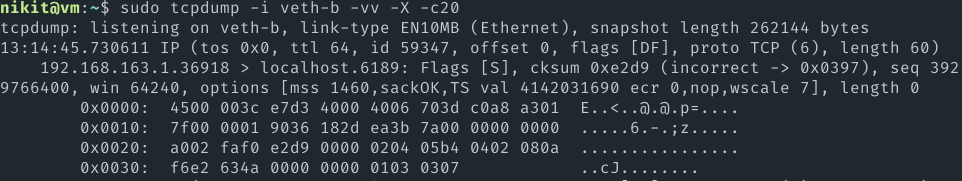
\includegraphics[width=\textwidth]{tcpdump.png}
  % \label{fig:result-png}
\end{figure}

\begin{Verbatim}[fontsize=\footnotesize,breaklines=true]
nikit@vm:~$ sudo tcpdump -i veth-b -vv -X -c20
tcpdump: listening on veth-b, link-type EN10MB (Ethernet), snapshot length 262144 bytes
13:14:45.730611 IP (tos 0x0, ttl 64, id 59347, offset 0, flags [DF], proto TCP (6), length 60)
    192.168.163.1.36918 > localhost.6189: Flags [S], cksum 0xe2d9 (incorrect -> 0x0397), seq 3929766400, win 64240, options [mss 1460,sackOK,TS val 4142031690 ecr 0,nop,wscale 7], length 0
        0x0000:  4500 003c e7d3 4000 4006 703d c0a8 a301  E..<..@.@.p=....
        0x0010:  7f00 0001 9036 182d ea3b 7a00 0000 0000  .....6.-.;z.....
        0x0020:  a002 faf0 e2d9 0000 0204 05b4 0402 080a  ................
        0x0030:  f6e2 634a 0000 0000 0103 0307            ..cJ........
13:14:45.730611 IP (tos 0x0, ttl 64, id 3198, offset 0, flags [DF], proto TCP (6), length 60)
    192.168.163.1.56888 > localhost.6187: Flags [S], cksum 0xe2d9 (incorrect -> 0x75b0), seq 2166629118, win 64240, options [mss 1460,sackOK,TS val 4142031690 ecr 0,nop,wscale 7], length 0
        0x0000:  4500 003c 0c7e 4000 4006 4b93 c0a8 a301  E..<.~@.@.K.....
        0x0010:  7f00 0001 de38 182b 8124 22fe 0000 0000  .....8.+.$".....
        0x0020:  a002 faf0 e2d9 0000 0204 05b4 0402 080a  ................
        0x0030:  f6e2 634a 0000 0000 0103 0307            ..cJ........
13:14:45.730617 IP (tos 0x0, ttl 64, id 47648, offset 0, flags [DF], proto TCP (6), length 60)
    192.168.163.1.59956 > localhost.6192: Flags [S], cksum 0xe2d9 (incorrect -> 0x4e62), seq 3750223847, win 64240, options [mss 1460,sackOK,TS val 4142031690 ecr 0,nop,wscale 7], length 0
        0x0000:  4500 003c ba20 4000 4006 9df0 c0a8 a301  E..<..@.@.......
        0x0010:  7f00 0001 ea34 1830 df87 dfe7 0000 0000  .....4.0........
        0x0020:  a002 faf0 e2d9 0000 0204 05b4 0402 080a  ................
        0x0030:  f6e2 634a 0000 0000 0103 0307            ..cJ........
13:14:45.734559 IP (tos 0x0, ttl 64, id 64801, offset 0, flags [DF], proto TCP (6), length 60)
    192.168.163.1.44176 > localhost.6188: Flags [S], cksum 0xe2d9 (incorrect -> 0x9029), seq 609785588, win 64240, options [mss 1460,sackOK,TS val 4142031694 ecr 0,nop,wscale 7], length 0
        0x0000:  4500 003c fd21 4000 4006 5aef c0a8 a301  E..<.!@.@.Z.....
        0x0010:  7f00 0001 ac90 182c 2458 96f4 0000 0000  .......,$X......
        0x0020:  a002 faf0 e2d9 0000 0204 05b4 0402 080a  ................
        0x0030:  f6e2 634e 0000 0000 0103 0307            ..cN........
13:14:45.734560 IP (tos 0x0, ttl 64, id 44301, offset 0, flags [DF], proto TCP (6), length 60)
    192.168.163.1.43544 > localhost.6191: Flags [S], cksum 0xe2d9 (incorrect -> 0xc277), seq 3038172764, win 64240, options [mss 1460,sackOK,TS val 4142031694 ecr 0,nop,wscale 7], length 0
        0x0000:  4500 003c ad0d 4000 4006 ab03 c0a8 a301  E..<..@.@.......
        0x0010:  7f00 0001 aa18 182f b516 d65c 0000 0000  ......./...\....
        0x0020:  a002 faf0 e2d9 0000 0204 05b4 0402 080a  ................
        0x0030:  f6e2 634e 0000 0000 0103 0307            ..cN........
13:14:45.734586 IP (tos 0x0, ttl 64, id 65371, offset 0, flags [DF], proto TCP (6), length 60)
    192.168.163.1.41570 > localhost.6190: Flags [S], cksum 0xe2d9 (incorrect -> 0x22b7), seq 1552275045, win 64240, options [mss 1460,sackOK,TS val 4142031694 ecr 0,nop,wscale 7], length 0
        0x0000:  4500 003c ff5b 4000 4006 58b5 c0a8 a301  E..<.[@.@.X.....
        0x0010:  7f00 0001 a262 182e 5c85 d665 0000 0000  .....b..\..e....
        0x0020:  a002 faf0 e2d9 0000 0204 05b4 0402 080a  ................
        0x0030:  f6e2 634e 0000 0000 0103 0307            ..cN........
13:15:18.754597 IP (tos 0x0, ttl 64, id 47649, offset 0, flags [DF], proto TCP (6), length 60)
    192.168.163.1.59956 > localhost.6192: Flags [S], cksum 0xe2d9 (incorrect -> 0xcd61), seq 3750223847, win 64240, options [mss 1460,sackOK,TS val 4142064714 ecr 0,nop,wscale 7], length 0
        0x0000:  4500 003c ba21 4000 4006 9def c0a8 a301  E..<.!@.@.......
        0x0010:  7f00 0001 ea34 1830 df87 dfe7 0000 0000  .....4.0........
        0x0020:  a002 faf0 e2d9 0000 0204 05b4 0402 080a  ................
        0x0030:  f6e2 e44a 0000 0000 0103 0307            ...J........
13:15:18.754603 IP (tos 0x0, ttl 64, id 3199, offset 0, flags [DF], proto TCP (6), length 60)
    192.168.163.1.56888 > localhost.6187: Flags [S], cksum 0xe2d9 (incorrect -> 0xf4af), seq 2166629118, win 64240, options [mss 1460,sackOK,TS val 4142064714 ecr 0,nop,wscale 7], length 0
        0x0000:  4500 003c 0c7f 4000 4006 4b92 c0a8 a301  E..<..@.@.K.....
        0x0010:  7f00 0001 de38 182b 8124 22fe 0000 0000  .....8.+.$".....
        0x0020:  a002 faf0 e2d9 0000 0204 05b4 0402 080a  ................
        0x0030:  f6e2 e44a 0000 0000 0103 0307            ...J........
13:15:18.754611 IP (tos 0x0, ttl 64, id 59348, offset 0, flags [DF], proto TCP (6), length 60)
    192.168.163.1.36918 > localhost.6189: Flags [S], cksum 0xe2d9 (incorrect -> 0x8296), seq 3929766400, win 64240, options [mss 1460,sackOK,TS val 4142064714 ecr 0,nop,wscale 7], length 0
        0x0000:  4500 003c e7d4 4000 4006 703c c0a8 a301  E..<..@.@.p<....
        0x0010:  7f00 0001 9036 182d ea3b 7a00 0000 0000  .....6.-.;z.....
        0x0020:  a002 faf0 e2d9 0000 0204 05b4 0402 080a  ................
        0x0030:  f6e2 e44a 0000 0000 0103 0307            ...J........
13:15:18.754611 IP (tos 0x0, ttl 64, id 65372, offset 0, flags [DF], proto TCP (6), length 60)
    192.168.163.1.41570 > localhost.6190: Flags [S], cksum 0xe2d9 (incorrect -> 0xa1ba), seq 1552275045, win 64240, options [mss 1460,sackOK,TS val 4142064714 ecr 0,nop,wscale 7], length 0
        0x0000:  4500 003c ff5c 4000 4006 58b4 c0a8 a301  E..<.\@.@.X.....
        0x0010:  7f00 0001 a262 182e 5c85 d665 0000 0000  .....b..\..e....
        0x0020:  a002 faf0 e2d9 0000 0204 05b4 0402 080a  ................
        0x0030:  f6e2 e44a 0000 0000 0103 0307            ...J........
13:15:18.758573 IP (tos 0x0, ttl 64, id 44302, offset 0, flags [DF], proto TCP (6), length 60)
    192.168.163.1.43544 > localhost.6191: Flags [S], cksum 0xe2d9 (incorrect -> 0x4177), seq 3038172764, win 64240, options [mss 1460,sackOK,TS val 4142064718 ecr 0,nop,wscale 7], length 0
        0x0000:  4500 003c ad0e 4000 4006 ab02 c0a8 a301  E..<..@.@.......
        0x0010:  7f00 0001 aa18 182f b516 d65c 0000 0000  ......./...\....
        0x0020:  a002 faf0 e2d9 0000 0204 05b4 0402 080a  ................
        0x0030:  f6e2 e44e 0000 0000 0103 0307            ...N........
13:15:18.758575 IP (tos 0x0, ttl 64, id 64802, offset 0, flags [DF], proto TCP (6), length 60)
    192.168.163.1.44176 > localhost.6188: Flags [S], cksum 0xe2d9 (incorrect -> 0x0f29), seq 609785588, win 64240, options [mss 1460,sackOK,TS val 4142064718 ecr 0,nop,wscale 7], length 0
        0x0000:  4500 003c fd22 4000 4006 5aee c0a8 a301  E..<."@.@.Z.....
        0x0010:  7f00 0001 ac90 182c 2458 96f4 0000 0000  .......,$X......
        0x0020:  a002 faf0 e2d9 0000 0204 05b4 0402 080a  ................
        0x0030:  f6e2 e44e 0000 0000 0103 0307            ...N........
13:15:23.874590 ARP, Ethernet (len 6), IPv4 (len 4), Request who-has 192.168.163.254 tell 192.168.163.1, length 28
        0x0000:  0001 0800 0604 0001 1ee8 7634 de23 c0a8  ..........v4.#..
        0x0010:  a301 0000 0000 0000 c0a8 a3fe            ............
13:15:23.874612 ARP, Ethernet (len 6), IPv4 (len 4), Reply 192.168.163.254 is-at 22:1e:d1:8a:df:f3 (oui Unknown), length 28
        0x0000:  0001 0800 0604 0002 221e d18a dff3 c0a8  ........".......
        0x0010:  a3fe 1ee8 7634 de23 c0a8 a301            ....v4.#....
13:16:07.906642 IP6 (hlim 255, next-header ICMPv6 (58) payload length: 16) fe80::1ce8:76ff:fe34:de23 > ip6-allrouters: [icmp6 sum ok] ICMP6, router solicitation, length 16
          source link-address option (1), length 8 (1): 1e:e8:76:34:de:23
            0x0000:  1ee8 7634 de23
        0x0000:  6000 0000 0010 3aff fe80 0000 0000 0000  `.....:.........
        0x0010:  1ce8 76ff fe34 de23 ff02 0000 0000 0000  ..v..4.#........
        0x0020:  0000 0000 0000 0002 8500 98ad 0000 0000  ................
        0x0030:  0101 1ee8 7634 de23                      ....v4.#
13:16:25.291232 IP (tos 0x0, ttl 64, id 26494, offset 0, flags [DF], proto TCP (6), length 60)
    192.168.163.1.35488 > localhost.6187: Flags [S], cksum 0xe2d9 (incorrect -> 0x445c), seq 2166629121, win 64240, options [mss 1460,sackOK,TS val 4142131250 ecr 0,nop,wscale 7], length 0
        0x0000:  4500 003c 677e 4000 4006 f092 c0a8 a301  E..<g~@.@.......
        0x0010:  7f00 0001 8aa0 182b 8124 2301 0000 0000  .......+.$#.....
        0x0020:  a002 faf0 e2d9 0000 0204 05b4 0402 080a  ................
        0x0030:  f6e3 e832 0000 0000 0103 0307            ...2........
13:16:25.291358 IP (tos 0x0, ttl 64, id 7858, offset 0, flags [DF], proto TCP (6), length 60)
    192.168.163.1.54732 > localhost.6192: Flags [S], cksum 0xe2d9 (incorrect -> 0xdddc), seq 3750223850, win 64240, options [mss 1460,sackOK,TS val 4142131251 ecr 0,nop,wscale 7], length 0
        0x0000:  4500 003c 1eb2 4000 4006 395f c0a8 a301  E..<..@.@.9_....
        0x0010:  7f00 0001 d5cc 1830 df87 dfea 0000 0000  .......0........
        0x0020:  a002 faf0 e2d9 0000 0204 05b4 0402 080a  ................
        0x0030:  f6e3 e833 0000 0000 0103 0307            ...3........
13:16:25.294655 IP (tos 0x0, ttl 64, id 25681, offset 0, flags [DF], proto TCP (6), length 60)
    192.168.163.1.33610 > localhost.6191: Flags [S], cksum 0xe2d9 (incorrect -> 0x6459), seq 3038172767, win 64240, options [mss 1460,sackOK,TS val 4142131254 ecr 0,nop,wscale 7], length 0
        0x0000:  4500 003c 6451 4000 4006 f3bf c0a8 a301  E..<dQ@.@.......
        0x0010:  7f00 0001 834a 182f b516 d65f 0000 0000  .....J./..._....
        0x0020:  a002 faf0 e2d9 0000 0204 05b4 0402 080a  ................
        0x0030:  f6e3 e836 0000 0000 0103 0307            ...6........
13:16:25.294677 IP (tos 0x0, ttl 64, id 14615, offset 0, flags [DF], proto TCP (6), length 60)
    192.168.163.1.55438 > localhost.6188: Flags [S], cksum 0xe2d9 (incorrect -> 0xdf3e), seq 609785591, win 64240, options [mss 1460,sackOK,TS val 4142131254 ecr 0,nop,wscale 7], length 0
        0x0000:  4500 003c 3917 4000 4006 1efa c0a8 a301  E..<9.@.@.......
        0x0010:  7f00 0001 d88e 182c 2458 96f7 0000 0000  .......,$X......
        0x0020:  a002 faf0 e2d9 0000 0204 05b4 0402 080a  ................
        0x0030:  f6e3 e836 0000 0000 0103 0307            ...6........
13:16:25.294752 IP (tos 0x0, ttl 64, id 11344, offset 0, flags [DF], proto TCP (6), length 60)
    192.168.163.1.57028 > localhost.6190: Flags [S], cksum 0xe2d9 (incorrect -> 0x6168), seq 1552275048, win 64240, options [mss 1460,sackOK,TS val 4142131254 ecr 0,nop,wscale 7], length 0
        0x0000:  4500 003c 2c50 4000 4006 2bc1 c0a8 a301  E..<,P@.@.+.....
        0x0010:  7f00 0001 dec4 182e 5c85 d668 0000 0000  ........\..h....
        0x0020:  a002 faf0 e2d9 0000 0204 05b4 0402 080a  ................
        0x0030:  f6e3 e836 0000 0000 0103 0307            ...6........
20 packets captured
21 packets received by filter
0 packets dropped by kernel
\end{Verbatim}

\subsection{Построить графики}

\noindent Парсим получаемый от утилиты вывод через python и выводим с помощью библиотеки pyplot.

\subsubsection*{Потребление программой cpu}

% \begin{figure}[h]
%   \centering
%   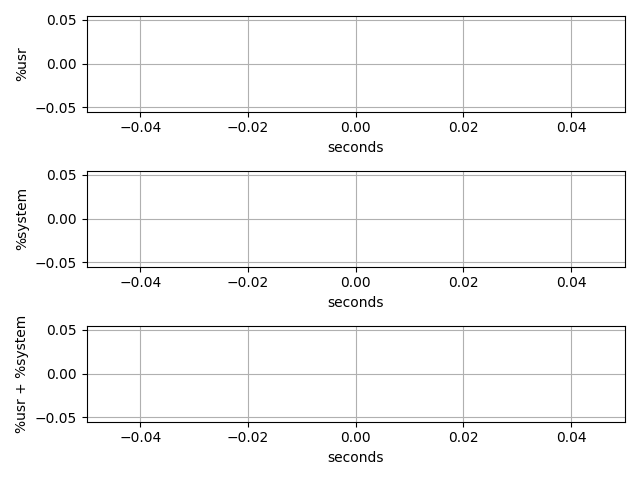
\includegraphics[width=0.7\textwidth]{fig-cpu.png}
%   % \label{fig:result-png}
% \end{figure}

\begin{figure}[h]
  \centering
  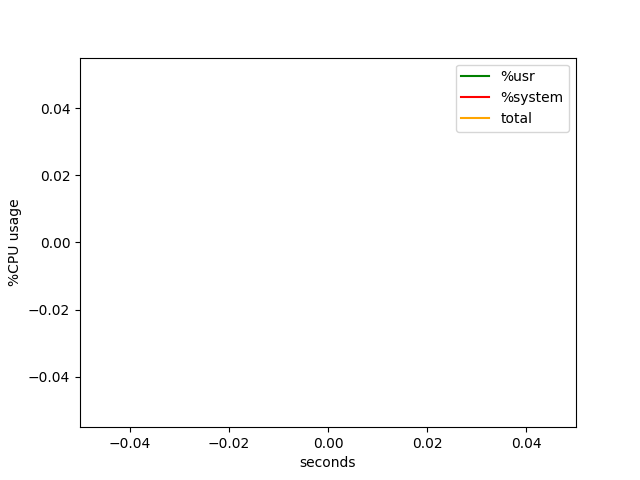
\includegraphics[width=0.7\textwidth]{fig-cpu-1.png}
  % \label{fig:result-png}
\end{figure}

\begin{figure}[h]
  \centering
  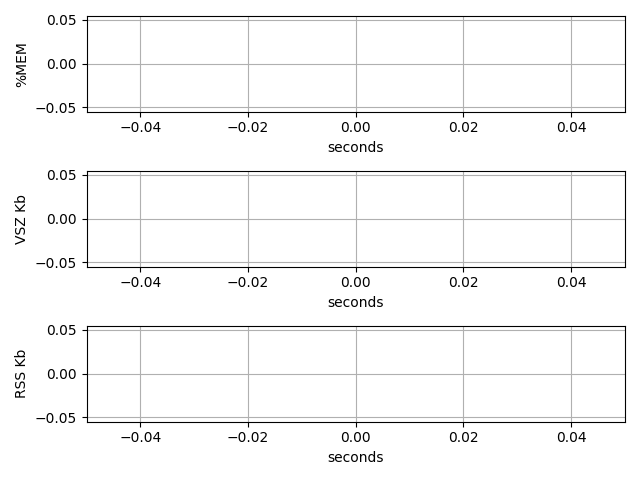
\includegraphics[width=0.7\textwidth]{fig-mem.png}
  % \label{fig:result-png}
\end{figure}

\newpage

\subsubsection*{Графики нагрузки генерируемой программой на подсистему ввода-вывода}

\begin{figure}[h]
  \centering
  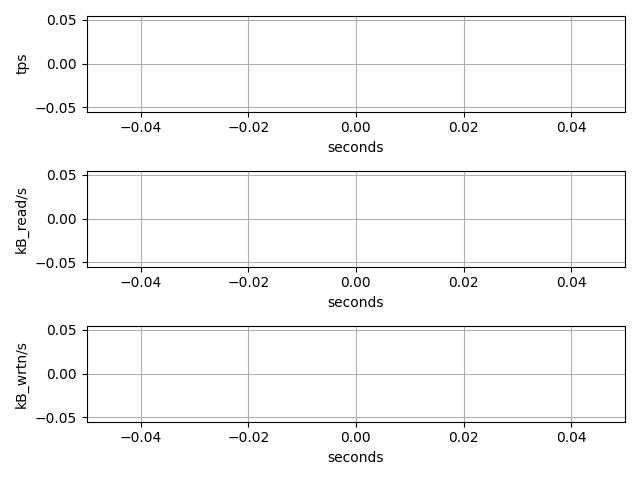
\includegraphics[width=0.7\textwidth]{fig-io.png}
  % \label{fig:result-png}
\end{figure}

\newpage

\subsubsection*{Графики нагрузки генерируемой программой на сетевую подсистему}

\begin{figure}[h]
  \centering
  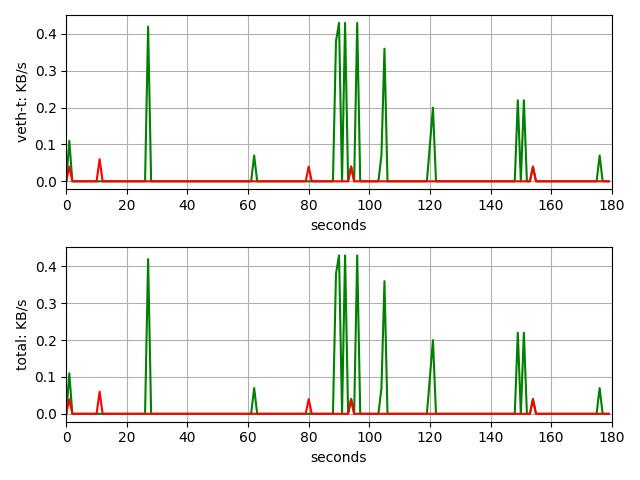
\includegraphics[width=0.7\textwidth]{fig-net.png}
  % \label{fig:result-png}
\end{figure}

\subsubsection*{Графики смены состояния исполнения потоков}

% \begin{figure}[h]
%   \centering
%   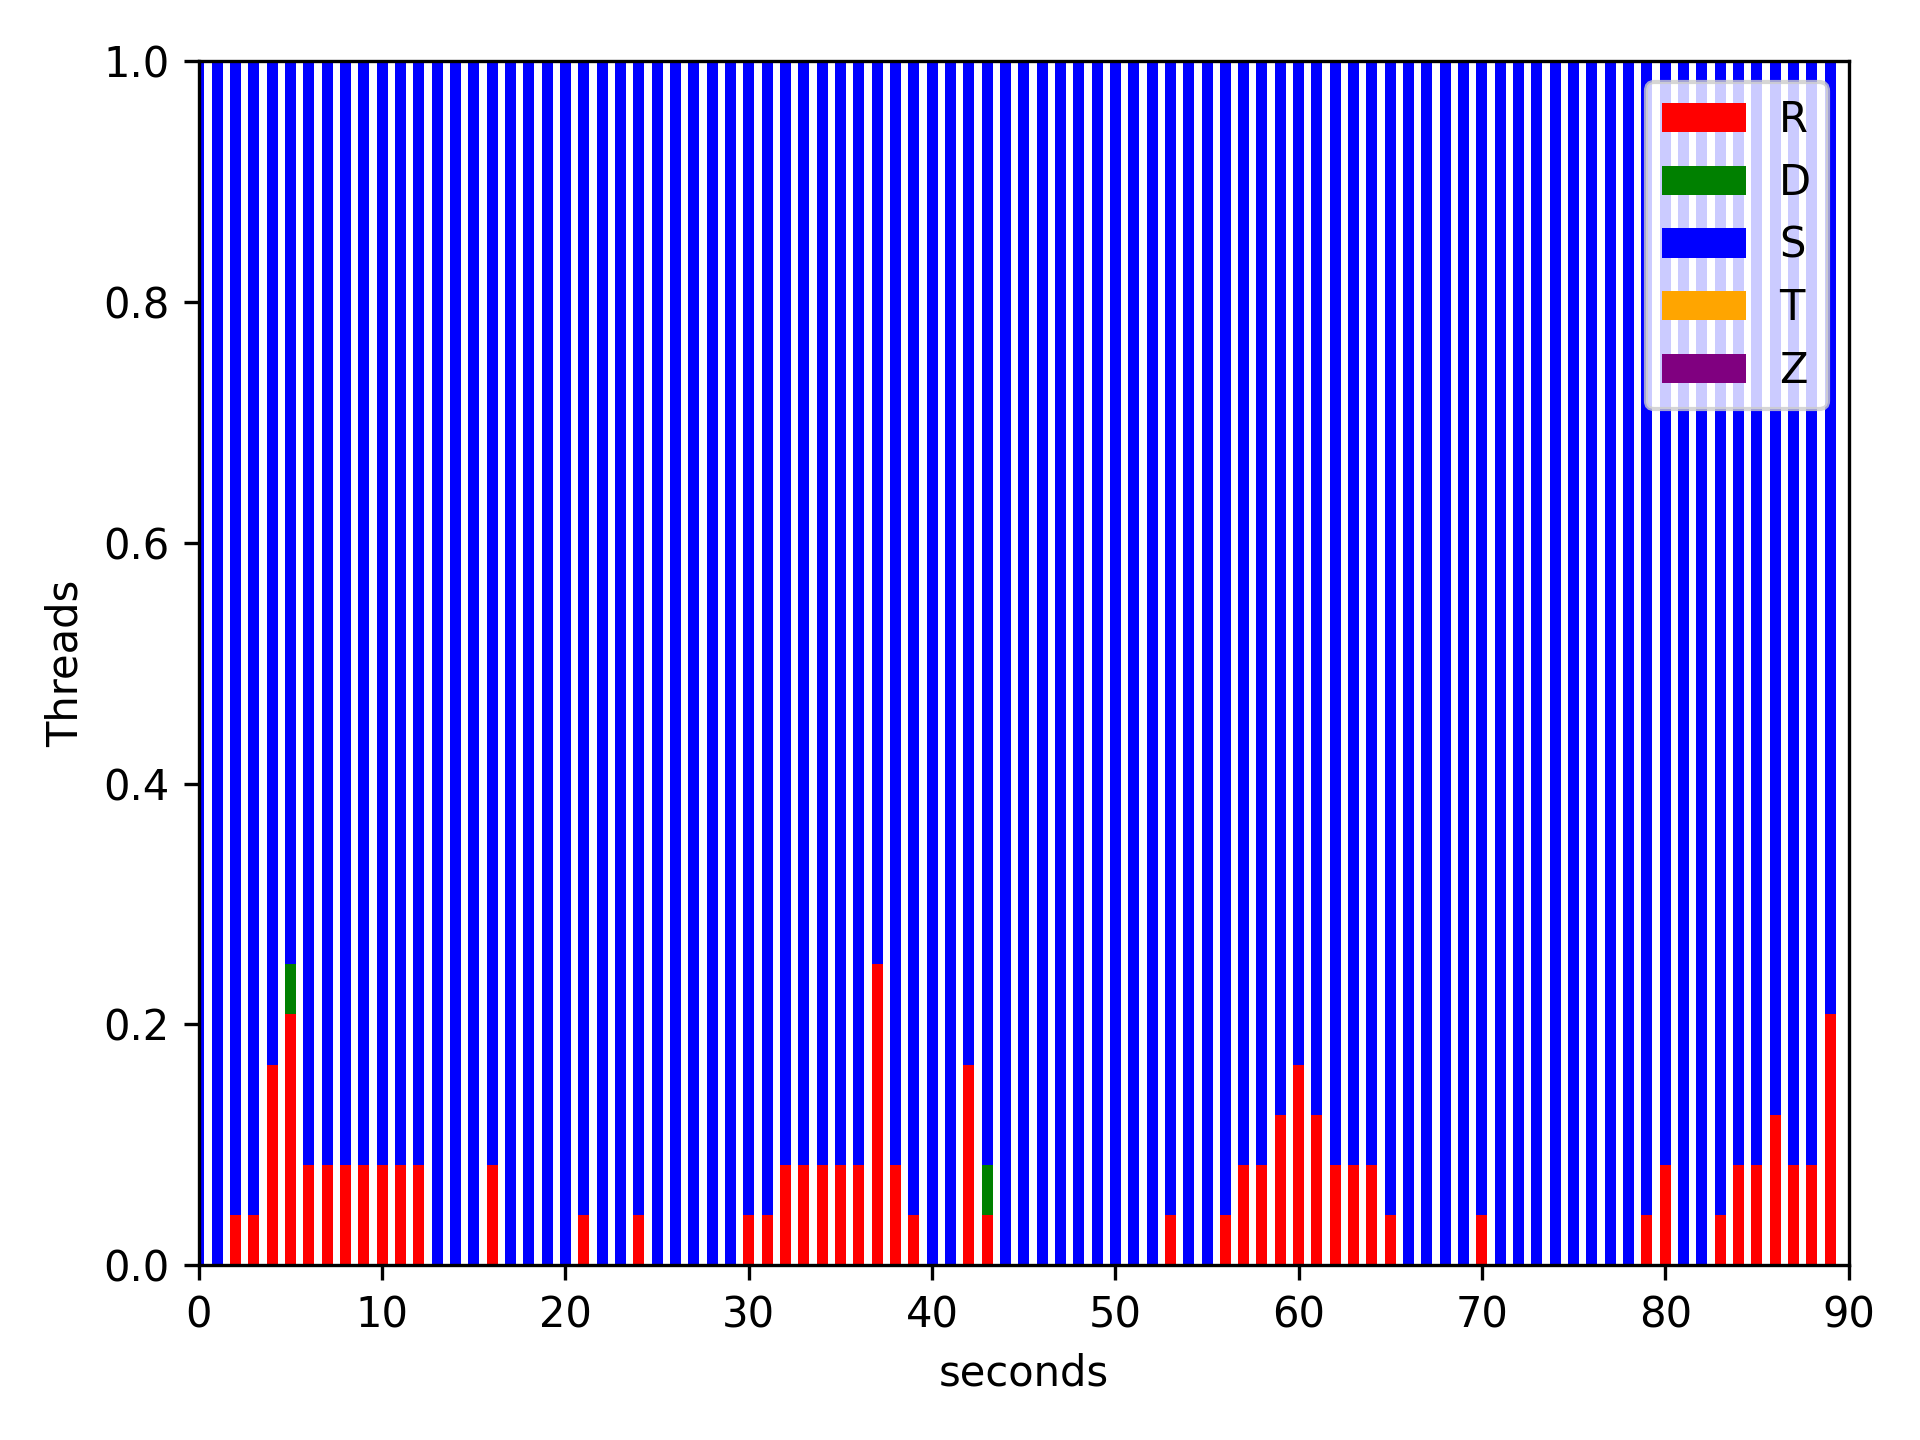
\includegraphics[width=0.7\textwidth]{fig-state.png}
%   % \label{fig:result-png}
% \end{figure}

\begin{figure}[h]
  \centering
  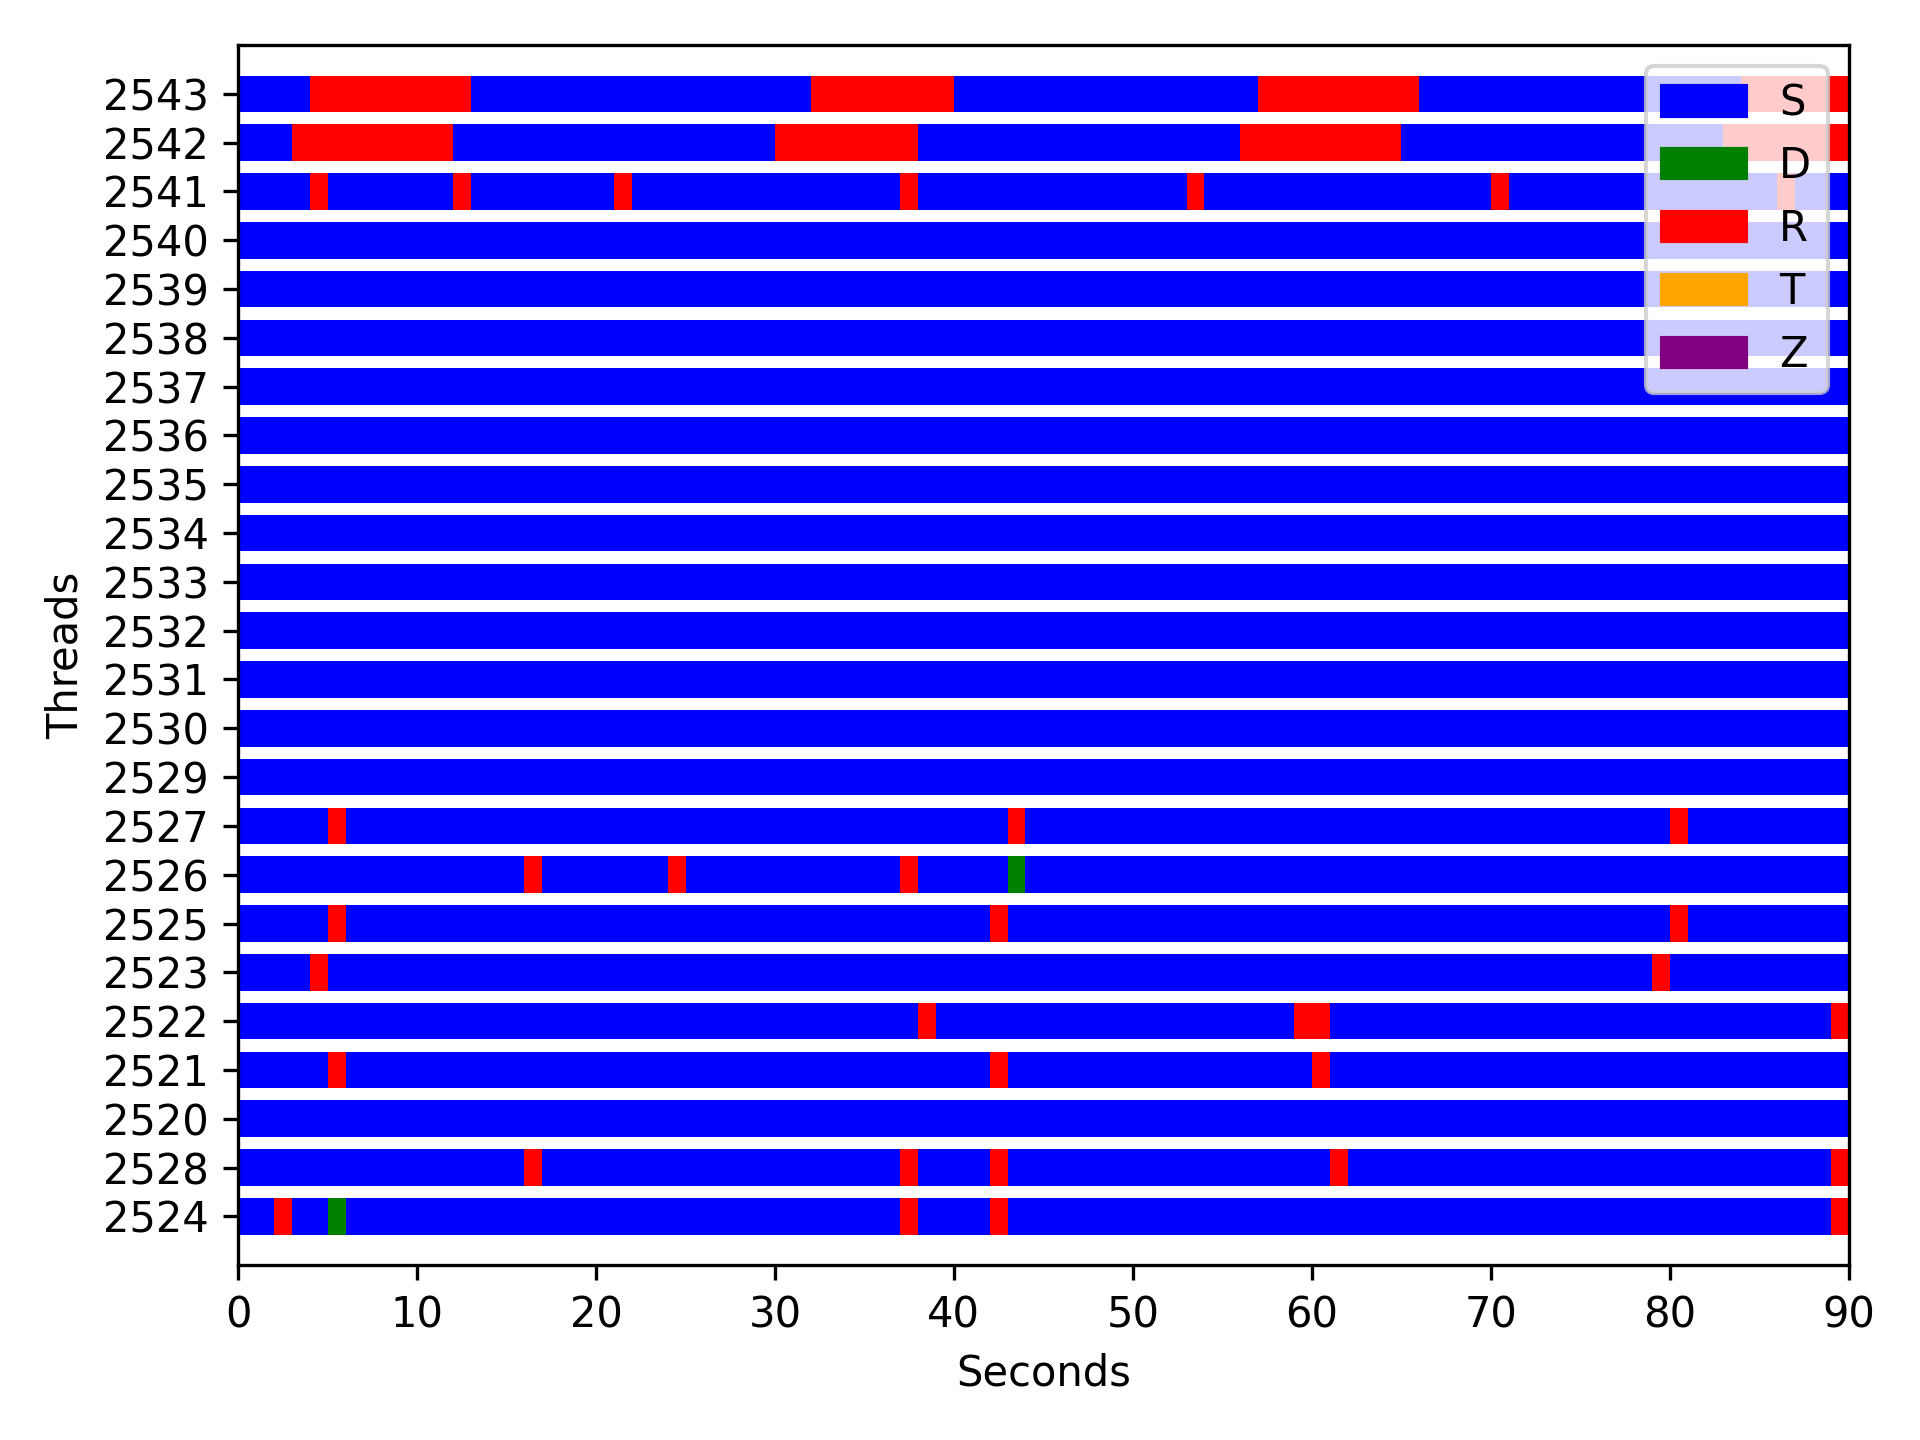
\includegraphics[width=0.7\textwidth]{fig-state-vert.png}
  % \label{fig:result-png}
\end{figure}

% \newpage

\section{Вывод}
В ходе выполнения лабораторной работы познакомился с утилитами, представленными выше, немного
поковырялся с сетями и неймспейсами, разобрался, как подключаться к виртуалке по ssh, скомпилировал
ядро по VirtualBox (gentoo moment), вспомнил, как парсить данные и строить графики на python.

\medskip
\noindent Исходный код исполняемых скриптов можно найти тут: 
\href{https://github.com/zubrailx/University-ITMO/tree/main/Year-3/Operating-systems/lab-1}{Последняя версия github репозитория}, 
или тут: \href{https://github.com/zubrailx/University-ITMO/tree/d290a6562783b7df35565233c4b5c3bb988bc2cd/Year-3/Operating-systems/lab-1}{Версия на момент сдачи}.

\end{document}
